\documentclass[11pt]{scrartcl}
\usepackage[utf8]{inputenc}
\usepackage{evank}


%% insert title here
\newcommand{\titlee}{Relativity I: Kinematics [Solutions]}
\parindent 0 pt

\newcommand{\officialsol}[1]{See the official solutions \href{#1}{here}.}

\title{\titlee}
\author{Cambridge Physics Academy}
\date{2023-2024}


\begin{document}

\thispagestyle{empty}
\begin{center}
    
    
    \Huge \textbf{\textsf{\titlee}}

    \large \theauthor
\end{center}

\setcounter{section}{-1}
\section{Readings}
\begin{itemize}
    \item Ch 11 of Morin
\end{itemize}
Feel free to do problems from the readings as extra practice.


\section{Lecture review}

\begin{defn}[Special Relativity]
    The posutlates of special relativity are:
    \begin{itemize}
        \item The speed of light is the same in any frame
        \item There is no preferred reference frame
    \end{itemize}
\end{defn}

\begin{theorem}[Fundamental Effects]
    From the postulates, we can derive the three fundamental effects:
    \begin{itemize}
        \item Time dilation: An observer A observes person B's time to be moving slower by a factor of $\gamma$.
        \item Length contraction: an observer sees lengths contracted by a factor of $\gamma$.
        \item Loss of simultaneity: simultaneity -- events happening at the same time -- is frame dependent.
    \end{itemize}
    where $\gamma = \frac{1}{\sqrt{1-v^2/c^2}}.$
\end{theorem}

\begin{theorem}[Lorentz Transformations]
    Let the frame $S'$ move with velocity $v\hat{\mathbf x}$ with respect to the frame of the observer, $S$. Then,
    $$x = \gamma (x' + vt'), t = \gamma (t'+vx'/c^2), \gamma = \frac{1}{\sqrt{1-v^2/c^2}}.$$
    This can also be written in matrix form,
    $$\begin{pmatrix}x\\ ct\end{pmatrix} = \begin{pmatrix} \gamma & \gamma \beta \\ \gamma \beta & \gamma \end{pmatrix}\begin{pmatrix}x'\\ ct'\end{pmatrix},$$
    where $\beta = v/c$. This can be made even simpler by setting $c = 1$.
\end{theorem}
\begin{theorem}[Invariant Interval]
    The quantity
    $$s^2 = (ct)^2 - x^2,$$
    known as the invariant interval, is invariant across Lorentz transformations. You won't see this used much in the olympiad, but the generalization of this -- the magnitude of any \href{https://en.wikipedia.org/wiki/Four-vector}{four-vector} will be introduced next week and be useful for energy and momentum.
\end{theorem}

\begin{theorem}
    If an object moves at velocity $v_2$ in frame $S'$ which moves at velocity $v_1$ with respect to frame $S$, then in frame $S$, the object moves at
    $$v = \frac{v_1 +v_2}{1+v_1v_2/c^2}.$$
\end{theorem}

Sometimes, spacetime diagrams, or minkowski diagrams, can be especially helpful for problem solving. They are graphs with a $t$ orc $ct$ vertical axis and $x$ as the horizontal axis, as shown below.
\begin{center}
    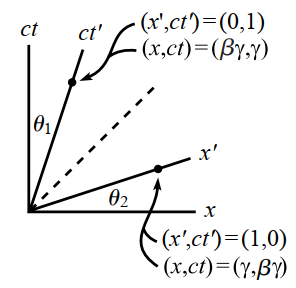
\includegraphics[width=4cm]{minky.png}
\end{center}
The $45$ degree line represents the path of light. One must be careful though, as the units scale differently:
$$\frac{\text{one }ct'\text{ unit}}{\text{one }ct\text{ unit}} = \frac{\text{one }x'\text{ unit}}{\text{one }x\text{ unit}} = \sqrt{\frac{1+\beta^2}{1-\beta^2}}$$

\begin{idea}[Rapidity]
    Rapidity, $\phi$ is defined by
    $$\tanh \phi = \beta = v/c.$$
    This is especially useful as the Lorentz transform becomes
    $$\begin{pmatrix}
 x \\ ct
\end{pmatrix} = \begin{pmatrix}\cosh \phi & \sinh \phi \\ \sinh \phi & \cosh \phi\end{pmatrix}\begin{pmatrix}x' \\ ct'\end{pmatrix},$$
analogous to a rotation in 2D. The velocity addition formula also becomes nicer, with
$$\tanh(\phi_1+\phi_2) = \frac{\tanh \phi_1 + \tanh \phi_2}{1+\tanh\phi_1 \tanh \phi_2}.$$
\end{idea}

\section{Problem Set}

\subsection{Exercises}

\begin{prob}
    In class, we briefly discussed the invariant interval $s^2 = (ct)^2 - x^2$. When can this quantity be less than $0$? When can this quantity be greater than $0$? What can this quantity say about the relative locations of the two events on a minkowski diagram?
\end{prob}
\begin{sol}
    This quantity can be less than 0 if the distance between two events is greater than $ct$, which means that they could not be traversed by one object -- it indicates a spacelike separation in any frame. When it is greater than $0$, it means the separation in distance is not as great and can be traversed by a single object -- it is timelike separation.

    If it is timelike, the segment formed by the two events forms an angle greater than $45^\circ$ above the horizontal, and if it is spacelike, the segment formed by the two events forms an angle less than $45^\circ$ above the horizontal.
\end{sol}

\begin{prob}[Morin]
    Two bombs lie on a train platform, a distance $L$ apart. As a train passes
by at speed $v$, the bombs explode simultaneously (in the platform frame)
and leave marks on the train. Due to the length contraction of the train,
we know that the marks on the train are a distance $\gamma L$ apart when viewed
in the train’s frame, because this distance is what is length-contracted
down to the given distance $L$ in the platform frame.
How would someone on the train quantitatively explain why the marks
are a distance $\gamma L$ apart, considering that the bombs are a distance of only
$L/\gamma$ apart in the train frame?
\end{prob}
\begin{sol}
    This is explained by the loss of simultaneity. Though the bombs explode simultaneously in the reference frame of the platform, they do not in the reference frame of the train.

Since the bombs explode simultaneously in the platform frame, we can imagine a light beam that starts from the center of the two bombs and explode when the light reaches them. In the reference frame of the train, the light reaches the front (closer to the front of the train) bomb first, since the ``gap closing" speed is $c+v$ and $c-v$ for the other one. So the first bomb explodes, and then the second bomb explodes after $\Delta t = \dfrac{L/2\gamma}{c-v}-\dfrac{L/2\gamma}{c+v}$. So in the reference frame of the train the distance between the two marks is
$$L/\gamma + v\Delta t = L/\gamma + v\cdot \dfrac{vL/\gamma}{c^2-v^2} = \dfrac{L}{\gamma}\left(1+\dfrac{v^2}{c^2 - v^2}\right)=\dfrac{L}{\gamma}\gamma^2 = L\gamma,$$
consistent with the platform frame.
\end{sol}

\begin{prob}[Morin]
    Cookie dough (chocolate chip, of course) lies on a conveyor belt that
moves at speed v. A circular stamp stamps out cookies as the dough
rushes by beneath it. When you buy these cookies in a store, what shape
are they? That is, are they squashed in the direction of the belt, stretched
in that direction, or circular?
\end{prob}
\begin{sol}
    The stamping is simultaneous in the lab frame, so this is the best frame to view it in. In this frame, the length contracted cookie fits in the stamp, which means that the real cookie is stretched in the direction of the belt.

    In the frame of the belt, the stamp does not come down simultaneously -- the back of it coming down first -- so it leads to a stretched stamping.
\end{sol}

\begin{prob}
    Suppose a source approaches you with speed $v$, emitting pulses of light at a frequency $f$ in its own frame. What is the frequency $f'$ at which these pulses reach you? This is the relativistic doppler effect.
\end{prob}
\begin{sol}
    The frequency $f$ means that there is a gap of $\Delta t = 1/f$ in the frame of the source. By time dilation, this results in a difference in time $\Delta t' = \gamma / f$ in your frame / the frame of the observer. But in our frame, the source continues moving, decreasing the space between the pulses. So, the space between the pulses in our frame is
    $$\Delta x = (c - v) \Delta t' = \gamma (c-v)/f.$$
    So, the perceived frequency on our end will be
    $$f' = \frac{c}{\Delta x} = \frac{c}{\gamma (c-v)} f = \sqrt{\frac{1+\beta}{1-\beta}}f.$$
\end{sol}

\begin{prob}
    Two balls move with speed $v$ along a line toward two people standing
along the same line. The proper distance between the balls is $\gamma L$, and
the proper distance between the people is $L$. Due to length contraction,
the people measure the distance between the balls to be $L$, so the balls
pass the people simultaneously (as measured by the people), as shown below. Assume that the people’s clocks both read zero at this time.
If the people catch the balls, then the resulting proper distance between
the balls becomes $L$, which is shorter than the initial proper distance of
$\gamma L$. Your task: By working in the frame in which the balls are initially at
rest, explain how the proper distance between the balls decreases from
$\gamma L$ to $L$. Do this in the following way
\begin{center}
    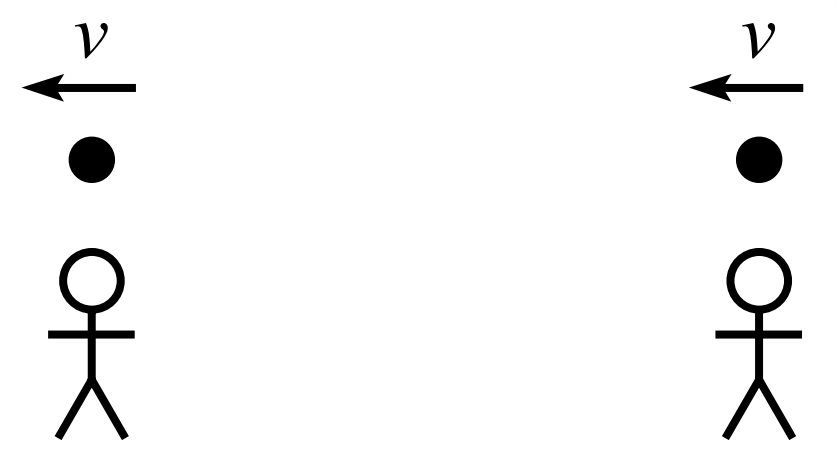
\includegraphics[width=5cm]{ball_pass.png}
\end{center}
\begin{anum}
    \item Draw the beginning and ending pictures for the process. Indicate
the readings on both clocks in the two pictures, and label all
relevant lengths.
\item Using the distances labeled in your pictures, how far do the people
travel? Using the times labeled in your pictures, how far do the
people travel? Show that these two methods give the same result.
\item Explain in words how the proper distance between the balls
decreases from $\gamma L$ to $L$.
\end{anum}
\end{prob}
\begin{alphasol}
    \item In the frame of the balls, the people are moving to the right with speed $v$. Furthermore, the rear clock is going to be ahead by $\Delta t = Lv/c^2$.
    \item After the rear person catches his ball first, the person in front goes a further distance of
    $$\Delta x = \gamma L - L/\gamma = \gamma L \left(1 - (1-v^2/c^2)\right) = \frac{\gamma Lv^2}{c^2}.$$
    By the clock, the front person goes further by
    $$\Delta x = \frac{\gamma Lv}{c^2}v,$$
    which is the same.
    \item The explanation is again loss of simultaneity! The rear person catches a ball first and brings it closer to the othe ball before the person in front catches their ball. 
\end{alphasol}

\begin{prob}
    Consider the Minkowski diagram below. In frame $S$, the hyperbola $c^2t^2 - x^2 = 1$ is drawn. Also drawn are the axes of frame $S'$,
which moves past $S$ with speed $v$. Use the invariance of the interval
$s^2 = c^2t^2 - x^2$ to derive the ratio of the unit sizes on the $ct'$ and $ct$ axes.
\begin{center}
    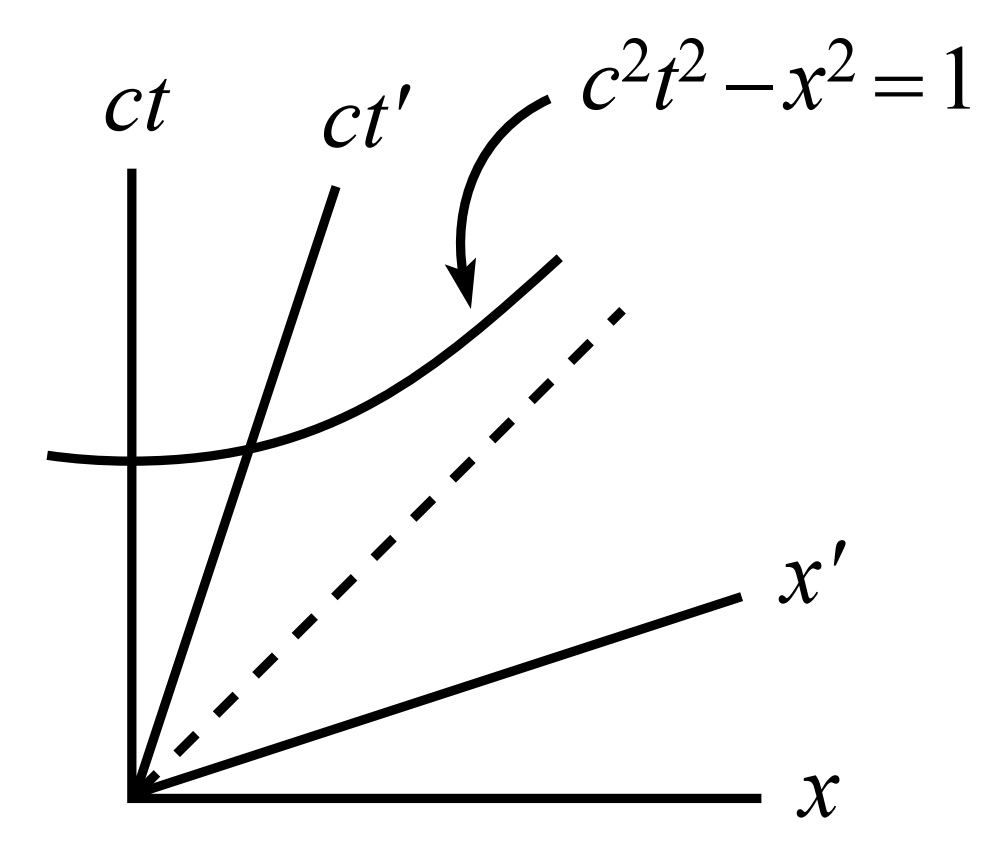
\includegraphics[width=4cm]{minkkkk.png}
\end{center}
\end{prob}
\begin{sol}
    By the invariant interval, the hyperbola must intersect both $ct = 1$ and $ct' = 1$. So, we can find the ratio of the unit sizes by simply finding the distances to the two intersection points. The $ct$ intersection point is of course just distance $1$. For $ct'$, we have $x = \beta (ct)$, so plugging into the hyperbola,
    $$\sqrt{1 - \beta^2}(ct) = 1,$$
    so thet total distance is
    $$\sqrt{(ct)^2 + x^2} = \sqrt{1+\beta^2} ct = \sqrt{\frac{1+\beta^2}{1-\beta^2}}.$$
\end{sol}

\begin{prob}
    \href{https://aapt.org/Common/upload/2020_USAPhO.pdf#page=5}{USAPhO 2020/A3}.
\end{prob}
\begin{sol}
    \officialsol{https://aapt.org/Common/upload/2020_USAPhO_solutions.pdf}
\end{sol}

\begin{prob}[Morin]
    Two spaceships float in space and are at rest relative to each other. They
are connected by a string. The string is strong, but it cannot withstand an arbitrary amount of stretching. At a given instant, the
spaceships simultaneously (with respect to their initial inertial frame)
start accelerating in the same direction (along the line between them)
with the same constant proper acceleration. In other words, assume
they bought identical engines from the same store, and they put them
on the same setting. Will the string eventually break?
\begin{center}
    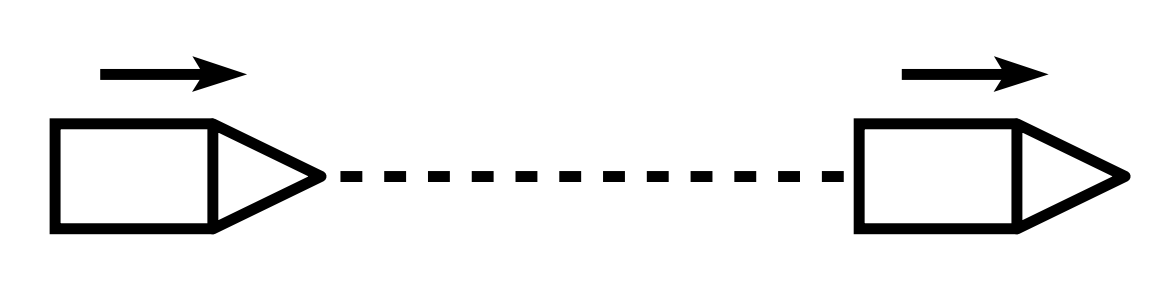
\includegraphics[width=5cm]{bellsparadox.png}
\end{center}
\end{prob}
\begin{sol}
    In the lab frame, their motion is symmetric, so they stay the same distance apart. However, that means that by length contraction, their distance in their own frames is increasing over time, and so this tells us that it breaks.

    How can we explain this in the frame of the rockets where it appears that the other rocket should stay still with respect to the other? They should both always be accelerating at the same time within the lab frame. However, if two events are simultaneous in the lab frame, by rear clock ahead, it must have happened earlier on the right side, and so the ship in front is accelerating slightly before the ship on the left, leading to the rope breaking.

    \href{https://www.youtube.com/watch?v=asW78vToNLQ}{Here} is a video explanation.
\end{sol}

\begin{prob}
    In class, we derived velocity as a function of \textit{proper} time for an object with constant proper acceleration. This time, we find it as a function of lab time.
    \begin{anum}
        \item By using the velocity addition formula, what is the acceleration in the lab frame as a function of time?
        \item Integrate your result from part (a) to find the object's velocity as a function of time.
        \item Lastly, integrate once more to get the object's position as a function of time. What does it look like on a minkowski diagram?
    \end{anum}
\end{prob}
\begin{alphasol}
    \item In the lab frame, we have by the velocity additino formula,
    $$v(t+dt) = \frac{v + a dt/\gamma}{1 +v adt/\gamma c^2} \approx v +\frac{adt}{\gamma} (1-\beta^2) = v + \frac{a dt}{\gamma ^3}. $$
    Thus, we have $\frac{dv}{dt} = \frac{adt}{\gamma^3}.$ 
    \item We can readily solve this differential equation,
    $$a t=  \int_0^v \gamma ^3 \, dv = \int_0^v \frac{1}{(1-\beta^2)^{3/2}} \, dv = \frac{v}{\sqrt{1 - \beta^2}}.$$
    Now, we can solve for $v$ in terms of $at$,  $$v(t) = \frac{at}{\sqrt{1 + (at/c)^2}}.$$
    \item Integrating $v(t)$ from $0$ to $t$, we get
    $$x(t) = \frac{c^2}{a}\left(\sqrt{1 + \left(\frac{at}{c}\right)^2} - 1\right)$$
    This is a hyperbola whose slope approaches the speed of light!
\end{alphasol}

\begin{prob}
    Suppose you have an object moving with 2-D velocity $\langle u_x',u_y'
    \rangle$ in frame $S'$, and frame $S'$ moves at velocity $\langle v,0\rangle$ with respect to frame $S$. What is the velocity of the object with respect to frame $S$? Follow a similar procedure from before to derive transverse velocity transformations.
\end{prob}
\begin{sol}
    The $y$ displacement in both frames should be the same,
    $$\Delta y = u_y'\Delta t'.$$
    By Lorentz transformations,
    $$\Delta t = \gamma \beta \Delta x' / c + \gamma  \Delta t'.$$
    In $S'$ we have $\Delta x' = u_x' \Delta t'$, so
    $$\frac{\Delta y}{\Delta t} = \frac{u_y'}{\gamma \beta u_x'/c + \gamma }= \boxed{\frac{u_y'/\gamma}{1 + \frac{v}{c^2}}}.$$
\end{sol}

\subsection{Challenge Problems}

\begin{prob}
    \href{https://apho.olimpicos.net/pdf/APhO_2013_Q2.pdf}{APhO 2013/T2}, a long relativistic kinematics question.
\end{prob}
\begin{sol}
    \officialsol{https://apho.olimpicos.net/pdf/APhO_2013_S2.pdf}
\end{sol}

\begin{prob}
    \href{https://drive.google.com/file/d/1HBcRaNfGWOYGUf1aMkmCK21Y77eAEU4i/view?usp=sharing}{IOAA 2022/T13}. This problem makes reference to energy and momentum at the start, but it can be done with just the \href{https://en.wikipedia.org/wiki/Relativistic_Doppler_effect}{relativistic doppler effect}. You can find a generalized version of the doppler effect that we derived earlier in the pset.
\end{prob}
\begin{sol}
    \officialsol{https://drive.google.com/file/d/1i3oIgC4eyskJXH9GdNj5VQacB8AXgxs2/view?usp=drive_link}
\end{sol}

\subsection{USAPhO Practice}

For the USAPhO practice this week, \textbf{set a 52.5 minute timer instead of the full hour} -- it will be a challenge but it will be reflective of the total time that was available in contest.

\begin{prob}[USAPhO 2021/A2]
    Alice the Mad Scientist, travelling in her flying car at height $h$ above the ground, shoots a beam of
muons at the ground. Bob, observing from the ground at distance $R \gg h$ from Alice’s car, decides
to check some facts about special relativity. Assume the muons travel extremely close to the speed
of light in Alice’s frame.
\begin{center}
    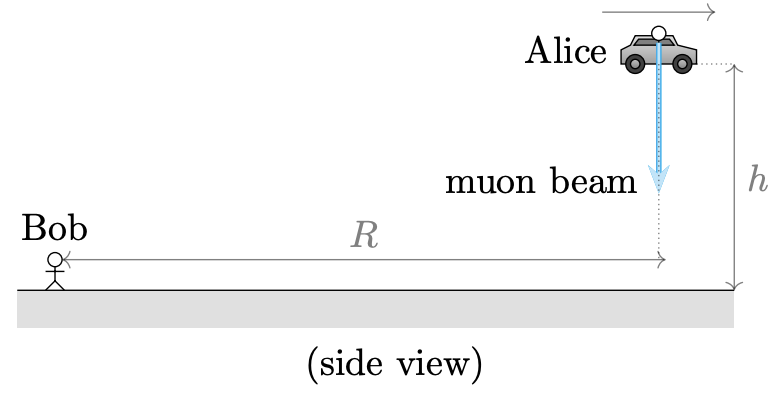
\includegraphics[width=6.5cm]{alicebob-1.png}
\end{center}
\begin{anum}
    \item Alice’s car flies at horizontal speed $v = \beta c$. Alice shoots her muon beam straight down, in her
reference frame. Express your answers in terms of $\beta, h , R$ and fundamental constants.
\begin{enumerate}[label=\roman*.]
    \item What is the horizontal velocity of the muons in Bob’s reference frame?
    \item What is the vertical velocity of the muons in Bob’s reference frame?
    \item How long does it take the muons to reach the ground in Bob’s reference frame?
\end{enumerate}

Alice’s velocity $v$ is directed an angle $\theta$ away from Bob. For the rest of the problem, you may additionally express your answers in terms of $\theta$.
\begin{center}
    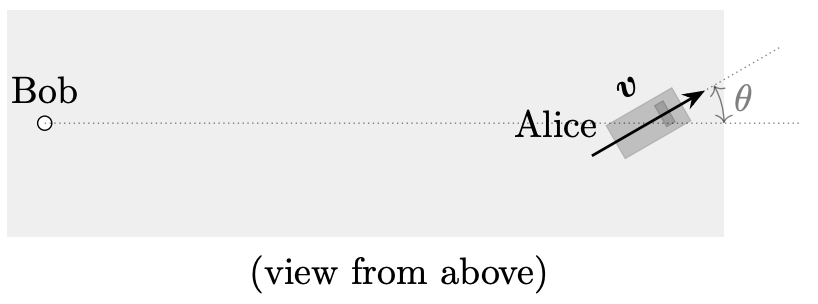
\includegraphics[width=6.5cm]{alicebob-2.png}
\end{center}
\item In Bob’s reference frame, how much time is there between when he sees Alice first fire the beam,
and when he sees the beam first hit the ground? (Hint: remember to account for the travel time
of light to Bob’s eyes.)
\item In this part, suppose that $\beta = 1/2$. Does there exist a value of $\theta$ so that the time it takes the
muons to hit the ground in Alice’s frame is equal to the time taken according to Bob’s eyes, in
Bob’s frame? If so, find the value of $\theta$ in degrees. If not, briefly explain why not.
\item Suppose Alice is carrying a radio transmitter set to frequency $f$. To what frequency would Bob
have to set his radio receiver in order to receive Alice’s transmission?
\end{anum}
\end{prob}
\begin{sol}
    \officialsol{https://aapt.org/Common2022/upload/2021-USAPhO.pdf}. Also, an old video solution by Evan \href{https://youtube.com/watch?v=hChVkXBqOHk}{here}.
\end{sol}

\begin{prob}
    \href{https://aapt.org/physicsteam/2016/upload/E3-2-3.pdf#page=5}{USAPhO 2016/A3} -- print out the answer sheets at the end.
\end{prob}
\begin{sol}
    \officialsol{https://aapt.org/physicsteam/2019/upload/USAPhO-2016-Solutions.pdf}
\end{sol}

\end{document}